\documentclass{siproblemset}

\usepackage{multicol}
\usepackage{xcolor}
\usepackage{mathtools}

% SI Session Information
\course{MTH 1321}
\sessionnum{PT1}
\sessiondate{9/19/19}

% Worksheet Information
\title{Practice Test \#1}
\sections{Sections 2.1-2.8}
\withnamespace

\definecolor{darkred}{RGB}{110,0,0}

%\debugmode

\begin{document}
    \maketitle
    
    \begin{center}
        \framebox{
            \begin{minipage}{\textwidth}
                \begin{center}
                    \textbf{When completing this practice test, do your best to mimic the test environment:}
                \end{center}
                \begin{enumerate}
                    \item Do not use a calculator.
                    \item Try not to use your notes.
                    \item Time yourself, make sure you are completing the problems at a comfortable pace. Remember that you will only get 75 mins for the actual exam (with fewer questions of course).
                \end{enumerate}
                \begin{center}
                    \color{darkred}\textbf{ Please do not share this practice test with anyone else. \underline{Your} commitment to SI and reviewing material earned this, not anyone else's.}
                \end{center}
                {\centering When you have finished the practice test, go to the following link to check your answers:\\ \color{blue}{https://forms.gle/Amfu2dUyx4MH1EmA8}\\}
            \end{minipage}
        }
    \end{center}

    % 1: Limit eval
    \begin{multipartquestion}
        Evaluate the following limits.
        \frq{$\lim\limits_{x\to1}\dfrac{x^2-2}{3x}$}
        \smallspace
        \frq{$\lim\limits_{x\to3}\dfrac{x^2-9}{x^2-2x-3}$}
        \smallspace
        \pagebreak
        \frq{$\lim\limits_{h\to0}\dfrac{\sqrt{7h+4}-2}{h}$}
        \smallspace
        \frq{$\lim\limits_{\theta\to0}\dfrac{3\theta\cot(2\theta)}{5}$}
        \smallspace
    \end{multipartquestion}

    % 2: Asymptotes
    \begin{multipartquestion}
        $f(x)=\dfrac{3x+2}{x^2-4x+4}$
        \frq{Determine all vertical asymptotes of $f(x)$. Use one or more limits to explain your answer.}
        \smallspace
        \frq{Determine one horizontal asymptote of $f(x)$. Use a limit to explain your answer.}
        \smallspace
    \end{multipartquestion}
    
    % 3: Continuity
    \pagebreak
    \frq{Use the definition of continuity to determine if $q(x)$ is continuous at $x=5$. Show your work or explain your answer. If $q$ is not continuous, find whether it is left- or right-continuous.}
    $$q(x)=\begin{cases}
        \dfrac{x-5}{|x-5|} & \text{, if } x\neq5\text; \\
        1 & \text{, if } x=5
    \end{cases}$$
    \mediumspace
    
    % 4: Limit eval
    \begin{multipartquestion}
        Evaluate the following limits algebraically.
        \frq{$\lim\limits_{x\to3}\dfrac{x-1}{x^2-3}$}
        \smallspace
        \frq{$\lim\limits_{x\to4}\dfrac{t^2-3t-4}{t^2-16}$}
        \smallspace
        \pagebreak
        \frq{$\lim\limits_{x\to-1}\dfrac{\sqrt{x^2+8}-3}{x+1}$}
        \smallspace
        \frq{$\lim\limits_{\theta\to0}\dfrac{3\tan(2\theta)}{4\theta}$}
        \smallspace
    \end{multipartquestion}

    % 5: Continuity
    \frq{Determine the value of $b$ that will make $r(x)$ continuous at $x=2$. Use the definition of continuity to explain your answer.}
    $$r(x)=\begin{cases}
    x^2-b & \text{, if } x<2\text; \\
    \cos(x^2-x-2) & \text{, if } x\geq2
    \end{cases}$$
    \largespace
    
    % 6: AROC
    \pagebreak
    \frq{What is the average rate of change of $f$ with respect to $x$ over the interval $[2,2+h]$? Simplify your answer as much as possible.}
    \[f(x)=\dfrac3x\]
    \largespace
    
    % 9: Limit eval
    \begin{multipartquestion}
        Evaluate the following limits algebraically.
        \frq{$\lim\limits_{x\to2}\dfrac{x-3}{16-x^2}$}
        \mediumspace
        \frq{$\lim\limits_{x\to3}\dfrac{x^3-9x}{x^2-x-6}$}
        \mediumspace
        \frq{$\lim\limits_{\theta\to0}3\csc(5\theta)\tan(2\theta)$}
        \mediumspace
    \end{multipartquestion}
    
    % 7: Limit/continuity from graph
    \begin{multipartquestion}
        Use the graph of g(x) below to answer the following questions.
        
        \mbox{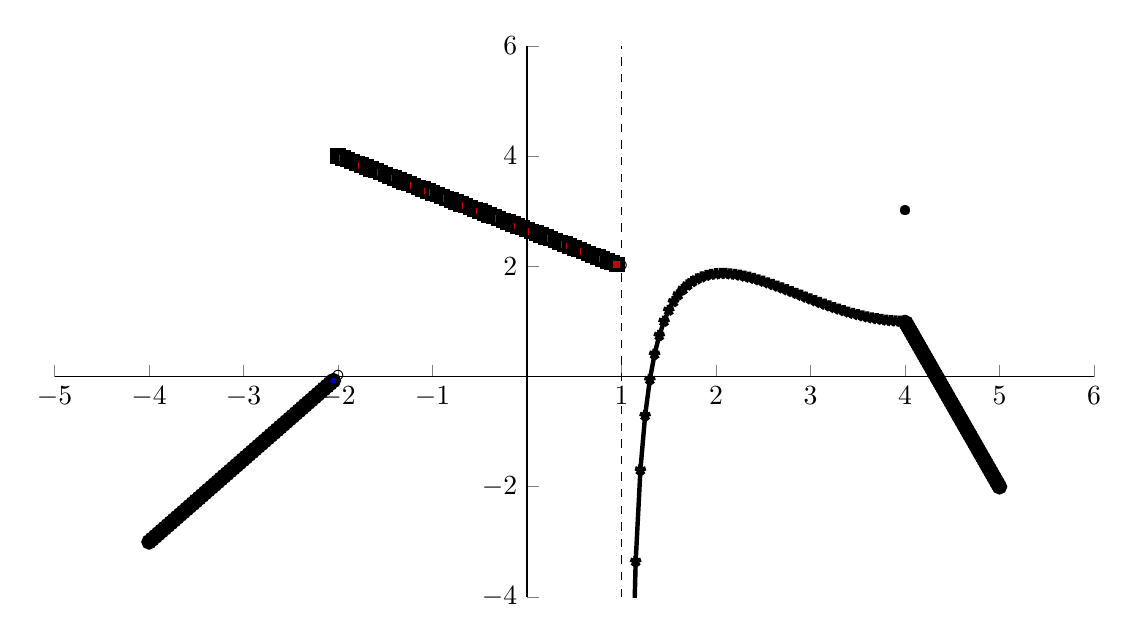
\begin{tikzpicture}[baseline=(current bounding box.north)]
            \begin{axis}[
            x=1.2cm,
            y=0.7cm,
            xmin=-5,
            xmax=6,
            ymin=-4,
            ymax=6,
            axis x line*=middle,
            axis y line*=middle,
            every axis plot/.append style={ultra thick},
            samples=60
            ]
            \addplot+[black, domain=-4:-2.05] {3/2*x+3};
            \addplot+[black, domain=-2:0.95] {-2/3*x+8/3};
            \addplot+[black, domain=4.01:5] {-3*x+13};
            \addplot+[black, domain=1:3.95, restrict y to domain =-10:10] {-1/(x-1)+cos(deg(x-1))+2.324};
            \node at (-2,0) {$\circ$};
            \node at (1,2) {$\circ$};
            \node at (4,1) {$\circ$};
            \node at (-2,4) {\textbullet};
            \node at (-4,-3) {\textbullet};
            \node at (5,-2) {\textbullet};
            \node at (4,3) {\textbullet};
            \draw[line width=0.25mm, dashed] ({axis cs:1,0}|-{rel axis cs:0,0}) -- ({axis cs:1,0}|-{rel axis cs:0,1});
            \end{axis}
            \end{tikzpicture}}
        \frq{$\lim\limits_{x\to-2}f(x)$}
        \nospace
        \frq{$\lim\limits_{x\to1^-}f(x)$}
        \nospace
        \frq{$\lim\limits_{x\to-4^+}f(x)$}
        \nospace
        \frq{Is $f(x)$ continuous at $x=4$? Use the definition of continuity to justify your answer.}
    \end{multipartquestion}

    % 8: Graph
    \pagebreak
    \mcq[1]{Draw the graph of a function f(x) with the following properties:}{
        \task $\lim\limits_{x\to-2^-}f(x)=-\infty$
        \task $\lim\limits_{x\to-2^+}f(x)=3$
        \task $\lim\limits_{x\to\infty}f(x)=3$
        \task $f(x)$ has the horizontal asymptote $y=2$
        \task $\lim\limits_{x\to3}f(x)$ exists, but $f(x)$ is not continuous at $x=3$
        \task $f(x)$ has a jump discontinuity at $x=-4$
    }
    \makebox[\width][c]{\begin{tikzpicture}[baseline=(current bounding box.north)]
        \begin{axis}[
        x=1.2cm,
        y=1.2cm,
        xmin=-6,
        xmax=6,
        ymin=-2,
        ymax=4,
        axis x line*=middle,
        axis y line*=middle,
        every axis plot/.append style={ultra thick},
        samples=60
        ]
        \end{axis}
        \end{tikzpicture}}
    
    % 10: Limit eval
    \begin{multipartquestion}
        Evaluate the following limits. Show work or briefly explain your answer.
        \frq{$\lim\limits_{x\to-\infty}\dfrac{3+e^x}{2e^x-5}$}
        \smallspace
        \frq{$\lim\limits_{x\to3^-}\dfrac{(x-2)(x-1)}{x-3}$}
        \smallspace
    \end{multipartquestion}

    
    % 11: Continuity
    \frq{Determine the value of $a$ that will make $g(x)$ continuous at $x=3$. Use the definition of continuity to explain your answer.}
    $$r(x)=\begin{cases}
        2^x+a & \text{, if } x<3\text; \\
        -\frac23x+5 & \text{, if } x\geq3
    \end{cases}$$
    \largespace
    
    % 12: IVT
    \frq{It is known that $f(x)$ is continuous on $[-2,2]$. Using the table below, show that $f(x)$ has a zero on $[-2,2]$. Explain your reasoning.}
    \begin{center}
        \begin{tabular}{|c|c|c|c|c|c|}
            \hline
            x & -2 & -1 & 0 & 1 & 2 \\
            \hline
            f(x) & 4 & 2 & 1 & -3 & 2 \\ 
            \hline
        \end{tabular}
    \end{center}

    % 13: Eval limits
    \pagebreak
    \begin{multipartquestion}
        Evaluate the following limits.
        \frq{$\lim\limits_{x\to-3}\dfrac{x^2-9}{x^2-2x-15}$}
        \mediumspace
        \frq{$\lim\limits_{x\to\infty}\dfrac{2x-\sqrt x}{x^2+2019}$}
        \mediumspace
        \frq{$\lim\limits_{x\to\infty}\left[\ln(3x+1)-\ln(2x+1)\right]$}
        \smallspace
    \end{multipartquestion}

    % 14: Limit stuff
    \pagebreak
    \begin{multipartquestion}
        Consider the graph of $f$ shown below.
        \begin{center}
            \mbox{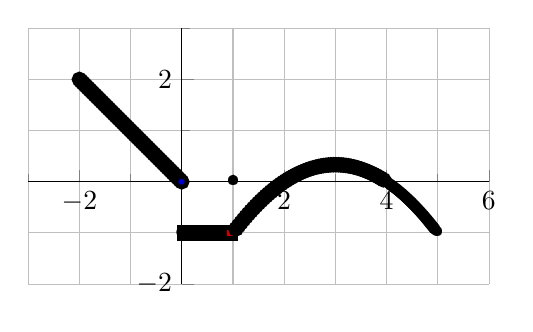
\begin{tikzpicture}[baseline=(current bounding box.north)]
                \begin{axis}[
                x=0.65cm,
                y=0.65cm,
                xmin=-3,
                xmax=6,
                ymin=-2,
                ymax=3,
                grid=both,
                major grid style={line width=.2pt,draw=gray!50},
                minor tick num=1,
                axis x line*=middle,
                axis y line*=middle,
                every axis plot/.append style={ultra thick},
                samples=60
                ]
                \addplot+[black, domain=-2:0] {-x};
                \addplot+[black, domain=0.06:0.94] {-1};
                \addplot+[black, domain=1.06:3.94] {-1/3*(x-3)^2+1/3};
                \addplot+[black, domain=4.06:4.94] {-1/3*(x-3)^2+1/3};
                \node at (-2,2) {$\circ$};
                \node at (0,-1) {$\circ$};
                \node at (1,-1) {$\circ$};
                \node at (4,0) {$\circ$};
                \node at (0,0) {\textbullet};
                \node at (1,0) {\textbullet};
                \node at (5,-1) {\textbullet};
                \end{axis}
                \end{tikzpicture}}
            
            Graph of $f$
        \end{center}
        \frq{Find all values of $a$ in $[-2, 5]$ such that $\lim\limits_{x\to a}f(x)=0$}
        \nospace
        \frq{Find all values of $b$ in $[-2, 5]$ such that $\lim\limits_{x\to b}f(x)=1$ or  $\lim\limits_{x\to b}f(x)=-1$}
        \nospace
        \frq{Is $f$ continuous at $x=1$? Explain why or why not.}
        \smallspace  
        \frq{Find the average rate of change of $f$ on the interval $[-2,0]$,}
        \smallspace
    \end{multipartquestion}
\end{document}